\myheader{Guía 4: Transformada de Fourier}


\begin{ejercicio}
    Hallar, utilizando propiedades, la transformada de Fourier de las siguientes señales:
    
    \begin{align*}
        \inciso & x(t) = 
        \begin{cases} 
            1 + \cos(\pi t) & |t| \leq 1 \\
            0 & |t| > 1 
        \end{cases} & \hspace{\fill} 
        \inciso & x(t) = \frac{\sin(\pi t)}{\pi t} \frac{\sin(2\pi (t-1))}{\pi (t-1)} \\
        \inciso & x(t) = 
        \begin{cases} 
            e^{-t} & 0 \leq t < 1 \\
            0 & \mbox{en otro caso}
        \end{cases} & \hspace{\fill} 
        \inciso & \parbox{.3\textwidth}{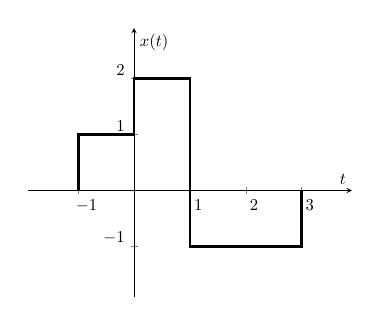
\begin{tikzpicture}[scale=0.6,transform shape]
    \begin{axis}[
    	axis y line=center,
    	axis x line=middle,
    	xlabel=$t$,ylabel=$x(t)$,
    	xmin=-1.9,xmax=3.9,
    	ymin=-1.9,ymax=2.9,
    	xticklabel style = {xshift=5},
    	yticklabel style = {yshift=5},
    	]
    	\addplot[
    	black,
    	ultra thick
    	] coordinates {
    	    (-1,0) (-1,1) (0,1) (0,2)
    	    (1,2) (1,-1) (3,-1) (3,0)
    	};
    \end{axis}
\end{tikzpicture}
} \\
        \inciso & \parbox{.3\textwidth}{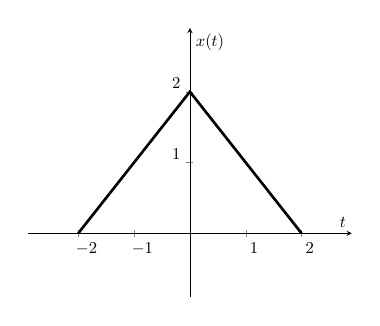
\begin{tikzpicture}[scale=0.6,transform shape]
    \begin{axis}[
    	axis y line=center,
    	axis x line=middle,
    	xlabel=$t$,ylabel=$x(t)$,
    	xmin=-2.9,xmax=2.9,
    	ymin=-0.9,ymax=2.9,
    	xticklabel style = {xshift=5},
    	yticklabel style = {yshift=5},
    	]
    	\addplot[
    	black,
    	ultra thick
    	] coordinates {
    	    (-2,0) (0,2) (2,0)
    	};
    \end{axis}
\end{tikzpicture}} & \hspace{\fill} 
        \inciso & \parbox{.3\textwidth}{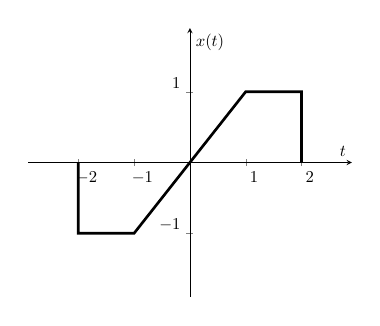
\begin{tikzpicture}[scale=0.6,transform shape]
    \begin{axis}[
    	axis y line=center,
    	axis x line=middle,
    	xlabel=$t$,ylabel=$x(t)$,
    	xmin=-2.9,xmax=2.9,
    	ymin=-1.9,ymax=1.9,
    	xticklabel style = {xshift=5},
    	yticklabel style = {yshift=5},
    	]
    	\addplot[
    	black,
    	ultra thick
    	] coordinates {
    	    (-2,0) (-2,-1) (-1,-1) (1,1) 
    	    (2,1) (2,0)
    	} ;
    \end{axis}
\end{tikzpicture}} \\
        \inciso & \parbox{.3\textwidth}{\begin{tikzpicture}[scale=0.6]
    \begin{axis}[
        x=.06\textwidth,y=0.1\textwidth,
    	axis y line=center,
    	axis x line=middle,
    	xlabel=$t$,ylabel=$x(t)$,
    	xmin=-7.9,xmax=7.5,
    	ymin=-0.3,ymax=2.3,
    	xticklabel style = {xshift=0},
    	yticklabel style = {yshift=5}
	]
	\diracdelta{-6}{2};
	\diracdelta{-5}{1};
	\diracdelta{-4}{2};
	\diracdelta{-3}{1};
	\diracdelta{-2}{2};
	\diracdelta{-1}{1};
	\diracdelta{0}{2};
	\diracdelta{1}{1};
	\diracdelta{2}{2};
	\diracdelta{3}{1};
	\diracdelta{4}{2};
	\diracdelta{5}{1};
	\node at (axis cs:6.5,1) {\Large $\cdots$} ;
	\node at (axis cs:-7,1) {\Large $\cdots$} ;
    \end{axis}
\end{tikzpicture}} & \hspace{\fill} & \\
    \end{align*}
    \end{ejercicio}
    
    \begin{ejercicio}
    Sea $x(t)$ la siguiente función:
    \begin{center}
        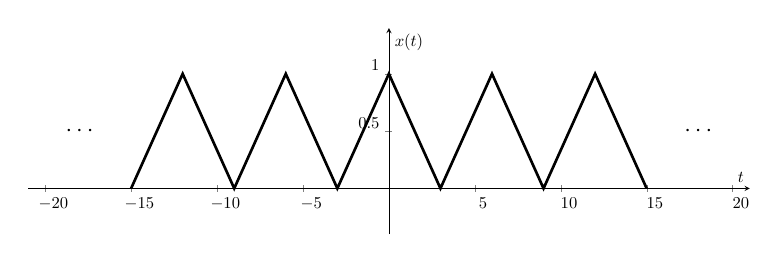
\begin{tikzpicture}[scale=0.6,transform shape]
    \begin{axis}[
        x=0.03\textwidth,y=0.2\textwidth,
    	axis y line=center,
    	axis x line=middle,
    	xlabel=$t$,ylabel=$x(t)$,
    	xmin=-21,xmax=21,
    	ymin=-0.4,ymax=1.4,
    	xticklabel style = {xshift=5},
    	yticklabel style = {yshift=5},
    	]
    	\addplot[
    	black,
    	ultra thick
    	] coordinates {
    	    (-15,0) (-12,1) 
    	    (-9,0) (-6,1)
    	    (-3,0) (0,1)
    	    (3,0) (6,1)
    	    (9,0) (12,1)
    	    (15,0)
    	};
    	\node at (18,0.5) {\Large $\cdots$} ;
    	\node at (-18,0.5) {\Large $\cdots$} ;
    \end{axis}
\end{tikzpicture}
    \end{center}
    
    \inciso Calcular la transformada de $x(t)$ utilizando la transformada $y(t) = \frac{\sin(\pi t)}{\pi t} \frac{\sin(2\pi (t-1))}{\pi (t-1)}$ calculada en el punto anterior. 
    
    \inciso ¿Qué relación existe entre la transformada de Fourier de una señal periódica y los coeficientes de su serie de Fourier? 
    
    \inciso ¿Qué característica distintiva tiene una Transformada de Fourier de una señal periódica?
    
    \end{ejercicio}
    
    
    \begin{ejercicio}
    Hallar, utilizando propiedades, la antitransformada de Fourier de las siguientes funciones:
    \begin{align*}
        \inciso & X(\omega) = \cos(4\omega + \pi/3) \\
        \inciso & X(\omega) = \frac{2\sin(3 (\omega-2\pi))}{\omega - 2\pi} \\
        \inciso & 
        X(\omega) \; \mathrm{tal\, que} \; |X(\omega)| = \begin{cases}
            |\omega| & \mbox{si } \omega \in [-1, 1) \\ 
            0 & \mathrm{en\, otro\, caso}
        \end{cases}
        \hspace*{1em} \mathrm{y} \hspace*{1em} \arg(X(\omega)) = -3\omega
    \end{align*}
    \end{ejercicio}
    
    \begin{ejercicio}
    Sea $X(\omega)$ la antitransformada de $x(t)$:
    \begin{center}
        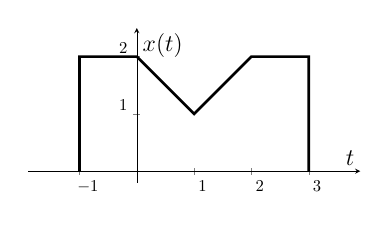
\begin{tikzpicture}[scale=0.6,transform shape]
    \begin{axis}[
        x=0.1\textwidth,y=0.1\textwidth,
    	axis y line=center,
    	axis x line=middle,
    	xlabel={\Large $t$},ylabel={\Large $x(t)$},
    	xmin=-1.9,xmax=3.9,
    	ymin=-0.2,ymax=2.5,
    	xtick distance=1,
    	ytick distance=1,
    	xticklabel style = {xshift=5},
    	yticklabel style = {yshift=5},
    	]
    	\addplot[
    	black,
    	ultra thick
    	] coordinates {
    	    (-1,0) (-1,2) (0,2) (1,1)
    	    (2,2) (3,2) (3,0)
    	};
    \end{axis}
\end{tikzpicture}

    \end{center}
    
    Hallar los siguientes valores sin obtener en forma explícita la función $X(\omega)$:
    \begin{align*}
        \inciso & \angle X(\omega) & \inciso & X(0) & \inciso & \int_{-\infty}^{\infty} X(\omega) d\omega \\[.5em]
        \inciso & \int_{-\infty}^{\infty} X(\omega) \frac{2\sin(\omega)}{\omega} e^{j2\omega} d\omega & \inciso & \int_{-\infty}^{\infty} |X(\omega)|^2 d\omega
    \end{align*}
    
    \end{ejercicio}
    
    \begin{ejercicio}
    Sea $x(t) = e^{-t} (u(t) - u(t-1))$. Graficar las siguientes funciones y hallar la transformada de Fourier de todas ellas:
    
    \inciso $x_1 = x(-t) + x(t) \hspace*{20em}$
    
    \inciso $x_2 = -x(-t) + x(t)$
    
    \inciso $x_3 = x(t+1) + x(t)$
    
    \inciso $x_4 = t x(t)$
    
    \end{ejercicio}
    
    \begin{ejercicio}
    Para cada una de las siguientes funciones
    \begin{align*}
        \inciso & \parbox{.5\textwidth}{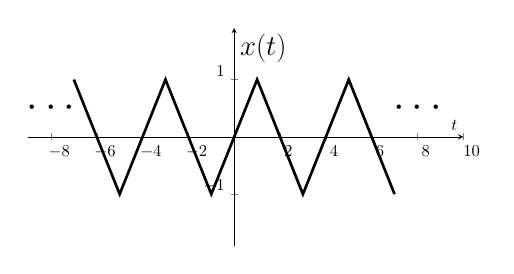
\begin{tikzpicture}[scale=0.6,transform shape]
    \begin{axis}[
        x=0.04\textwidth,y=0.1\textwidth,
    	axis y line=center,
    	axis x line=middle,
    	xlabel=$t$,ylabel={\LARGE $x(t)$},
    	xmin=-9,xmax=10,
    	ymin=-1.9,ymax=1.9,
    	xticklabel style = {xshift=5},
    	yticklabel style = {yshift=5},
    	]
    	\addplot[
    	black,
    	ultra thick
    	] coordinates {
    	    (-7,1) (-5,-1) 
    	    (-3,1) (-1,-1)
    	    (1,1) (3,-1)
    	    (5,1) (7,-1)
    	};
    	\node at (8,0.5) {\Huge $\cdots$} ;
    	\node at (-8,0.5) {\Huge $\cdots$} ;
    \end{axis}
\end{tikzpicture}} & \hspace{\fill} &
        \inciso & \parbox{.3\textwidth}{\begin{tikzpicture}[scale=0.6,transform shape]
    \begin{axis}[
    	axis y line=center,
    	axis x line=middle,
    	xlabel=$t$,ylabel=$x(t)$,
    	xmin=-2.9,xmax=2.9,
    	ymin=-0.9,ymax=2.9,
    	xticklabel style = {xshift=5},
    	yticklabel style = {yshift=5},
    	]
    	\diracdelta{1}{2};
    \end{axis}
\end{tikzpicture}} \\
        \inciso & \parbox{.5\textwidth}{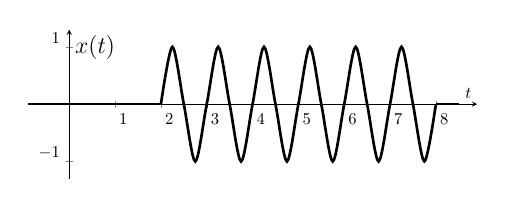
\begin{tikzpicture}[scale=0.6,transform shape]
    \begin{axis}[
        x=0.08\textwidth,y=0.1\textwidth,
    	axis y line=center,
    	axis x line=middle,
    	xlabel=$t$,ylabel={\Large $x(t)$},
    	xmin=-0.9,xmax=8.9,
    	ymin=-1.3,ymax=1.3,
    	xticklabel style = {xshift=5},
    	yticklabel style = {yshift=5},
    	]
    	\addplot [
    	black, ultra thick,
    	domain=2:8, smooth
    	] {sin(deg(2*pi*x))} ;
    	\addplot[
    	black, ultra thick
    	] coordinates {(-1,0) (2,0)} ;
    	\addplot[
    	black, ultra thick
    	] coordinates {(8,0) (8.5,0)} ;
    \end{axis}
\end{tikzpicture}} & \hspace{\fill} &
        \inciso & \parbox{.3\textwidth}{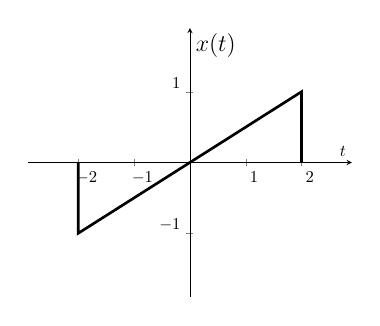
\begin{tikzpicture}[scale=0.6,transform shape]
    \begin{axis}[
    	axis y line=center,
    	axis x line=middle,
    	xlabel=$t$,ylabel={\Large $x(t)$},
    	xmin=-2.9,xmax=2.9,
    	ymin=-1.9,ymax=1.9,
    	xticklabel style = {xshift=5},
    	yticklabel style = {yshift=5},
    	]
    	\addplot[
    	black,
    	ultra thick
    	] coordinates {(-2,0) (-2,-1) (2,1) (2,0)} ;
    \end{axis}
\end{tikzpicture}} \\
        \inciso & \parbox{.5\textwidth}{\pgfmathdeclarefunction{ejcuatrotresa}{1}{%
  \pgfmathparse{#1^2 * exp(-abs(#1))}%
}

\begin{tikzpicture}[scale=0.6,transform shape]
    \begin{axis}[
        x=0.04\textwidth,y=0.2\textwidth,
    	axis y line=center,
    	axis x line=middle,
    	xlabel=$t$,ylabel={\Large $x(t)=t^2 e^{-|t|}$},
    	xmin=-8.9,xmax=8.9,
    	ymin=-.3,ymax=1.3,
    	xticklabel style = {xshift=5},
    	yticklabel style = {yshift=5},
    	samples=100
    	]
    	\addplot [
    	black, ultra thick,
    	domain=-10:10, smooth
    	] {ejcuatrotresa(x)} ;
    \end{axis}
\end{tikzpicture}} & \hspace{\fill} &
        \inciso & \parbox{.3\textwidth}{\pgfmathdeclarefunction{gauss}{3}{%
  \pgfmathparse{exp(-((#1-#2)^2)/(2*#3^2))}%
}

\begin{tikzpicture}[scale=0.6,transform shape]
    \begin{axis}[
        x=0.04\textwidth,y=0.2\textwidth,
    	axis y line=center,
    	axis x line=middle,
    	xlabel=$t$,ylabel={\Large $x(t)=e^{-t^2/2}$},
    	xmin=-4.9,xmax=4.9,
    	ymin=-.3,ymax=1.3,
    	xticklabel style = {xshift=5},
    	yticklabel style = {yshift=5},
    	]
    	\addplot [
    	black, ultra thick,
    	domain=-10:10, smooth, samples=100
    	] {gauss(x,0,1)} ;
    \end{axis}
\end{tikzpicture}} \\
    \end{align*}
    indicar si cumplen algunas de estas condiciones:
    \begin{itemize}
        \item $\Realpart{X(\omega)} = 0$
        \item $\Impart{X(\omega)} = 0$
        \item $\exists \alpha \in \mathbb{R}$ tal que $e^{j\omega\alpha}X(\omega)$ es una función real
        \item $\int_{-\infty}^{\infty} X(\omega) d\omega = 0$
        \item $\int_{-\infty}^{\infty} \omega X(\omega) d\omega = 0$
        \item $X(\omega)$ es periódica
    \end{itemize}
    
    \end{ejercicio}
    
    \begin{ejercicio}
    Hallar y graficar la transformada de Fourier de tiempo discreto de las siguientes secuencias:
    
    \inciso $x(n) = u(n) - u(n-20)$
    
    \inciso $x(n) = \delta(n) - \delta(n-1)$
    
    \inciso $x(n) = \left( \frac{1}{2} \right)^{-n} u(-n-1)$
    
    \inciso $x(n) = \sin\left(\frac{\pi}{2} n \right) + \cos(n)$
    \end{ejercicio}
    
    \begin{ejercicio}
    Segunda parte del ejercicio 6a de la guía vieja. No entiendo qué hay que hacer.
    \end{ejercicio}
    
    \begin{ejercicio}
    Hallar la antitransformada de Fourier en tiempo discreto de las siguientes funciones:
    
    \inciso $X(e^{j\Omega}) = 1 + 3e^{-j2\Omega} - 4e^{-j10\Omega}$
    
    \inciso $X(e^{j\Omega}) = \sum_{k=-\infty}^{\infty} (-1)^k \delta(\Omega - \frac{\pi}{2}k)$
    
    \inciso $X(e^{j\Omega}) = \frac{e^{-j\Omega} - 1/5}{1-1/5 e^{-j\Omega}}$
    \end{ejercicio}
    
    \begin{ejercicio}
    Sea $X(e^{j\Omega})$ la antitransformada de Fourier de la secuencia $x(n)$:
    
    \begin{center}
    \parbox{.7\textwidth}{\begin{tikzpicture}[scale=0.6]
    \begin{axis}[
        x=.06\textwidth,y=0.1\textwidth,
    	axis y line=center,
    	axis x line=middle,
    	xlabel=$n$,ylabel=$x(n)$,
    	xmin=-7.9,xmax=11.9,
    	ymin=-1.3,ymax=2.3,
    	xticklabel style = {xshift=0},
    	yticklabel style = {yshift=5}
	]
	\discretedelta{-7}{0.1};
	\discretedelta{-6}{0.1};
	\discretedelta{-5}{0.1};
	\discretedelta{-4}{0.1};
	\discretedelta{-3}{-1};
	\discretedelta{-2}{0.1};
	\discretedelta{-1}{1};
	\discretedelta{0}{2};
	\discretedelta{1}{1};
	\discretedelta{2}{0.1};
	\discretedelta{3}{1};
	\discretedelta{4}{2};
	\discretedelta{5}{1};
	\discretedelta{6}{0.1};
	\discretedelta{7}{-1};
	\discretedelta{8}{0.1};
	\discretedelta{9}{0.1};
	\discretedelta{10}{0.1};
	\discretedelta{11}{0.1};
    \end{axis}
\end{tikzpicture}}
    \end{center}
    
    Hallar los siguientes valores sin obtener explícitamente la función $X(e^{j\Omega})$:
    \begin{align*}
    \inciso & X(0) & \inciso & \angle X(e^{j\Omega}) & \inciso & \int_{-\pi}^{\pi} X(e^{j\Omega}) d\Omega \\ 
    \inciso & X(e^{j\pi}) & \inciso & \int_{-\pi}^{\pi}  \left|\frac{X(e^{j\Omega})}{d\Omega}\right|^2 d\Omega &
    \end{align*}
    \end{ejercicio}
    
    
    \begin{ejercicio}
    Para cada una de las siguientes funciones
    \begin{align*}
        \inciso & \parbox{.3\textwidth}{\begin{tikzpicture}[scale=0.6,transform shape]
    \begin{axis}[
        x=0.04\textwidth,y=0.1\textwidth,
    	axis y line=center,
    	axis x line=middle,
    	xlabel=$n$,ylabel={\LARGE $x(n)$},
    	xmin=-4.9,xmax=8.9,
    	ymin=-0.3,ymax=2.9,
    	xticklabel style = {xshift=0},
    	yticklabel style = {yshift=5},
    	]
    	\discretedelta{-4}{0.1};
    	\discretedelta{-3}{0.1};
    	\discretedelta{-2}{0.1};
    	\discretedelta{-1}{0.5};
    	\discretedelta{0}{1};
    	\discretedelta{1}{1.5};
    	\discretedelta{2}{2};
    	\discretedelta{3}{1.5};
    	\discretedelta{4}{1};
    	\discretedelta{5}{0.5};
    	\discretedelta{6}{0.1};
    	\discretedelta{7}{0.1};
    	\discretedelta{8}{0.1};
    \end{axis}
\end{tikzpicture}} &
        \inciso & \parbox{.4\textwidth}{\begin{tikzpicture}[scale=0.6,transform shape]
    \begin{axis}[
        x=0.04\textwidth,y=0.1\textwidth,
    	axis y line=center,
    	axis x line=middle,
    	xlabel=$n$,ylabel={\LARGE $x(n)$},
    	xmin=-9.9,xmax=9.9,
    	ymin=-1.3,ymax=1.9,
    	xticklabel style = {xshift=0},
    	yticklabel style = {yshift=5},
    	]
    	\discretedelta{-8}{0.1};
    	\discretedelta{-7}{-1};
    	\discretedelta{-6}{0.1};
    	\discretedelta{-5}{1};
    	\discretedelta{-4}{0.1};
    	\discretedelta{-3}{-1};
    	\discretedelta{-2}{0.1};
    	\discretedelta{-1}{1};
    	\discretedelta{0}{0.1};
    	\discretedelta{1}{-1};
    	\discretedelta{2}{0.1};
    	\discretedelta{3}{1};
    	\discretedelta{4}{0.1};
    	\discretedelta{5}{-1};
    	\discretedelta{6}{0.1};
    	\discretedelta{7}{1};
    	\discretedelta{8}{0.1};
    	\node at (-9,0.5) {\Large $\cdots$};
    	\node at (9,0.5) {\Large $\cdots$};
    \end{axis}
\end{tikzpicture}} \\
        \inciso & \parbox{.3\textwidth}{\begin{tikzpicture}[scale=0.6,transform shape]
    \begin{axis}[
        x=0.03\textwidth,y=0.1\textwidth,
    	axis y line=center,
    	axis x line=middle,
    	xlabel=$n$,ylabel={\LARGE $x(n)$},
    	xmin=-9.9,xmax=9.9,
    	ymin=-1.3,ymax=2.9,
    	xticklabel style = {xshift=0},
    	yticklabel style = {yshift=5},
    	]
    	\discretedelta{-9}{0.1};
    	\discretedelta{-8}{0.1};
    	\discretedelta{-7}{0.1};
    	\discretedelta{-6}{0.1};
    	\discretedelta{-5}{0.1};
    	\discretedelta{-4}{-1};
    	\discretedelta{-3}{-1};
    	\discretedelta{-2}{0.1};
    	\discretedelta{-1}{0.1};
    	\discretedelta{0}{2};
    	\discretedelta{1}{-1};
    	\discretedelta{2}{0.1};
    	\discretedelta{3}{0.1};
    	\discretedelta{4}{1};
    	\discretedelta{5}{0.1};
    	\discretedelta{6}{0.1};
    	\discretedelta{7}{0.1};
    	\discretedelta{8}{0.1};
    \end{axis}
\end{tikzpicture}} &
        \inciso & \parbox{.4\textwidth}{\begin{tikzpicture}[scale=0.6,transform shape]
    \begin{axis}[
        x=0.04\textwidth,y=0.1\textwidth,
    	axis y line=center,
    	axis x line=middle,
    	xlabel=$n$,ylabel={\LARGE $x(n)$},
    	xmin=-9.9,xmax=9.9,
    	ymin=-1.3,ymax=2.9,
    	xticklabel style = {xshift=0},
    	yticklabel style = {yshift=5},
    	]
    	\discretedelta{-9}{0.1};
    	\discretedelta{-8}{0.1};
    	\discretedelta{-7}{0.1};
    	\discretedelta{-6}{2};
    	\discretedelta{-5}{0.1};
    	\discretedelta{-4}{-1};
    	\discretedelta{-3}{-1};
    	\discretedelta{-2}{0.1};
    	\discretedelta{-1}{1};
    	\discretedelta{0}{0.1};
    	\discretedelta{1}{1};
    	\discretedelta{2}{0.1};
    	\discretedelta{3}{-1};
    	\discretedelta{4}{-1};
    	\discretedelta{5}{0.1};
    	\discretedelta{6}{2};
    	\discretedelta{7}{0.1};
    	\discretedelta{8}{0.1};
    	\discretedelta{9}{0.1};
    \end{axis}
\end{tikzpicture}} 
    \end{align*}
    indicar si cumplen algunas de estas condiciones:
    \begin{itemize}
        \item $\Realpart{X(e^{j\Omega})} = 0$
        \item $\Impart{X(e^{j\Omega})} = 0$
        \item $\exists \alpha \in \mathbb{R}$ tal que $e^{j\Omega\alpha}X(e^{j\Omega})$ es una función real
        \item $\int_{-\pi}^{\pi} X(e^{j\Omega}) d\Omega = 0$
        \item $X(e^{j\Omega})$ es periódica
        \item $X(e^{j\Omega})|_{\Omega=0} = 0$
    \end{itemize}
    \end{ejercicio}
    
    \begin{ejercicio}
    Considere un sistema LTI discreto cuya respuesta al impulso es $h(n) = \left(\frac{1}{2}\right)^n u(n)$. Usando la transformada de Fourier de tiempo discreto hallar la salida $y(n)$ para las siguientes entradas:
    
    \inciso $x(n) = \left(\frac{3}{4}\right)^n u(n)$
    
    \inciso $x(n) = \left(-1\right)^n u(n)$
    
    \inciso $x(n) = A e^{j\frac{\pi}{2}n},\; -\infty < n < \infty$
    
    \inciso $x(n) = 10 - 5 \sin\left(\frac{\pi}{2} n\right) + 20 \cos(\pi n),\; -\infty < n < \infty$
    
    \end{ejercicio}
    
    \begin{ejercicio}
    Para el sistema descripto por la ecuación en diferencias $y(n) = \frac{1}{2} y(n-1) + x(n)$ con condiciones iniciales de reposo, se pide:
    
    \inciso Encontrar la expresión analítica de la salida $y(n)$ ante una entrada $x(n)$ aplicada a partir de $n = 0$.
    
    \inciso Encontrar a partir de la expresión anterior la salida que corresponde cuando la entrada es $x(n) = \delta(n)$. 
    
    \inciso Encontrar a partir de la expresión general de la salida del sistema, la salida que corresponde
    cuando la entrada es $x(n) = A e^{j\frac{\pi}{2}n}, n \geq 0$. A partir de esta expresión, y
    comparándola con la obtenida en el ejercicio anterior (c) discuta el significado de la respuesta permanente y de la transitoria. Grafique ambos tipos de respuesta mediante MATLAB. Discuta qué función de MATLAB utilizaría para obtener la respuesta del sistema, \texttt{conv} o \texttt{filter}.
    
    \end{ejercicio}
    
    \begin{ejercicio}
    Este ejercicio pide transformar las funciones del ejercicio 7a (guía vieja) y volver a hacerlo de vuelta. Hay que reformularlo de manera más imaginativa. 
    \end{ejercicio}